%!TEX program = xelatex
\documentclass[9pt, compress]{beamer}
\usetheme[titleprogressbar]{m}

\usepackage{booktabs}  
\usepackage[scale=2]{ccicons}
\usepackage{minted}
\usepgfplotslibrary{dateplot}
\usemintedstyle{trac}
\author{\textbf{Rania Sayed}, \textbf{Hazem Al Saied} } 
\title{The research system in Germany}
%\subtitle{}
%\logo{}
\institute{\textbf{Uinversité de Lorraine}}
\date{October 2015}
%\subject{}
%\setbeamercovered{transparent}
%\setbeamertemplate{navigation symbols}{}
\begin{document}
	\maketitle
	\begin{frame}
		\frametitle{Outlines}
		\tableofcontents{}
	\end{frame}
\section{Introduction}
	\begin{frame}
		\frametitle{Introduction}
		\begin{itemize}
		    \item Germany has one of the largest research systems in the OECD
			\item there are nearly 1,000 public   funded institutions of science, research and development in Germany
			 
		\end{itemize}
	\end{frame}

	\begin{frame} %BilantInfo
		\frametitle{Introduction 2}
		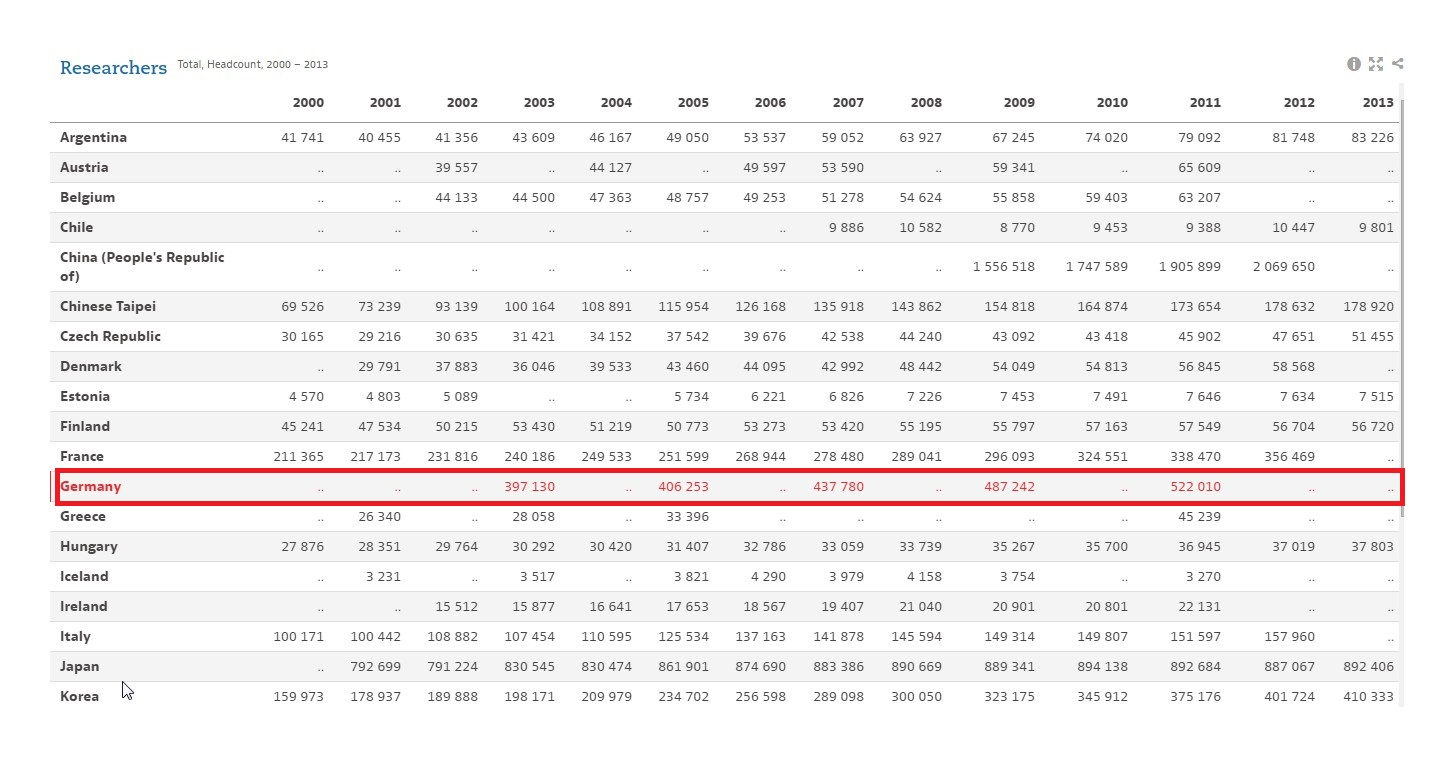
\includegraphics[width=\textwidth,height=300pt]{img/no_researchers.jpg}
		
	\end{frame}
	\section{Overview of the German research system}
	\begin{frame} 
		\frametitle{Overview of the German research system}
		\begin{figure}
        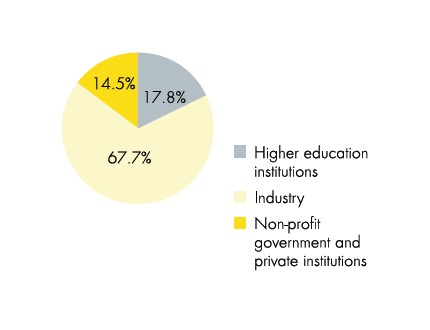
\includegraphics[width=\textwidth,height=150pt]{img/R_org_graph.jpg}
        \caption{Distribution of budget on different sectors}
		\end{figure}
	\end{frame}
	
	\begin{frame} 
		\frametitle{Overview of the German research system}
		
			Public funding for different aspects of research is organised in one of three ways: 
			\begin{itemize}
			\item From federal sources (e.g. project funding); 
            \item From state sources (e.g. institutional funding for higher education
institutions, state R\&D institutions); 
            \item Jointly from federal and state sources according to agreed formula (e.g.institutional funding of public research institutes of national significance; project funding for universities;categories of research infrastructure).
		\end{itemize}
	
	\end{frame}
	\section{Research Organisations}
	\begin{frame} 
		\frametitle{Research Organisations}
		\begin{figure}
		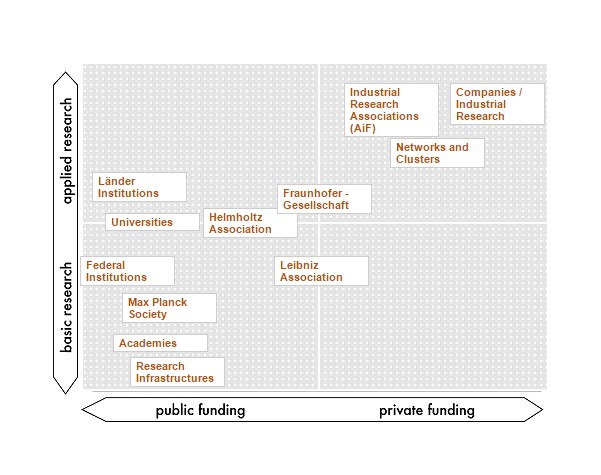
\includegraphics[width=\textwidth,height=175pt]{img/ResearchOrg.jpg}
		\caption{Overview of research-performing organisations in Germany}
		\end{figure}
	\end{frame}
	\subsection{Public research institutes}
	\begin{frame} 
		\frametitle{Public research institutes}
		
			Public research institutes are  organised into four large networks:
			\begin{itemize}
			\item The Max Planck Gesellschaft (MPG) 
            \item The Fraunhofer Gesellschaft (FhG)
            \item The Helmholtz-Gemeinschaft Deutscher Forschungszentren (HGF) 
            \item The Wissenschaftsgemeinschaft Wilhelm-Gottfried-Leibniz (WGL)
		\end{itemize}
	\end{frame}
	\subsection{Research Activities}
	\begin{frame} 
			\frametitle{Research Activities}
		
			\centering
		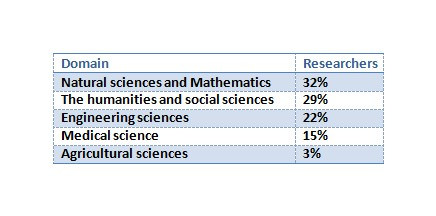
\includegraphics[scale=0.7]{img/Domain_Res.jpg}
	\end{frame}

	\section{Research Funding System }
	\begin{frame} 
		\frametitle{Funding types in Germany}
		\begin{itemize}
			\item\textbf{ Government Funding}
				\begin{itemize}
					\item more than 390 public universities and colleges are funded by the Länder.
				\end{itemize}
		\end{itemize}
	
			\begin{itemize}
				\item\textbf{ The European Funding}
			\end{itemize}
			\begin{itemize}
				\item\textbf{ The Industrial Funding}
							\begin{itemize}
								\item  In 2012, German companies  spending amounted to a total of 2.5 billion euros.
							\end{itemize}
			\end{itemize}

	\end{frame}
	\begin{frame} 
		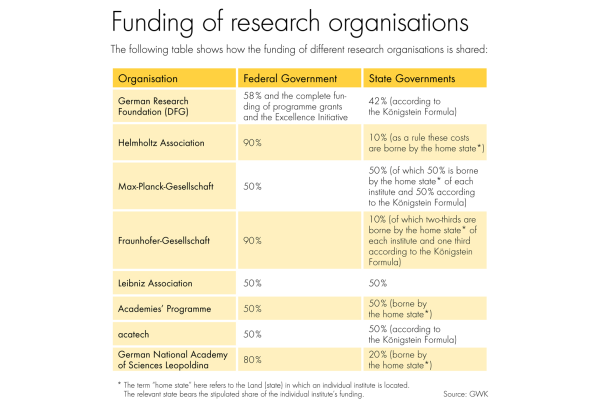
\includegraphics[width=\textwidth,height=175pt]{img/FundingoResearch.png}
		\newline
		\centering
		Figure Shows the collaboration between the federal and states governments.
	\end{frame}

	\section{PHD Student }
	\begin{frame} 
		\frametitle{PHD Student}
		\begin{quotation}
			4,000 international graduates complete their doctorate in Germany every year.
		\end{quotation}
		\begin{itemize}
			\item five reasons to do your PhD in Germany:
			\begin{enumerate}
				\setcounter{enumi}{0}
				\item Outstanding reputation of German doctorate
				\item Strong international focus: PhD in English
				\item Good funding opportunities 
				\item Excellent research infrastructure
				\item High standard of living			
			\end{enumerate}
		\end{itemize}
	\end{frame}
	\subsection{Ways to do th PHD in Germany}
	\begin{frame} 
		\frametitle{Ways to do the PHD in Germany}
		\begin{enumerate}
			\setcounter{enumi}{0}
			\item \textbf{Individual Doctorate}
			\begin{itemize}
				\item Involves the thesis produced under the supervision of a professor. 
				\item Three to five years are normal. 
			\end{itemize}
			\item \textbf{Structured PhD Programs}
			\begin{itemize}
				\item A team of supervisors look after a group of doctoral students. 
				\item The duration of  studies is  limited to three years.
			\end{itemize}
		\end{enumerate} 
	\end{frame}
	\subsection{Computer science} 
	\begin{frame} 
		\frametitle{Computer science}
		programs and organizations  each PhD student should know :
		\begin{enumerate}
			\setcounter{enumi}{0}
			\item \textbf{Bitkom}
			\begin{itemize}
				\item  Represent more than 2,300 companies in the digital economy.
			\end{itemize}
			\item \textbf{BMBF} 
			\begin{itemize}
				\item Drives more than 80 per cent of innovations in Germany.
			\end{itemize}
			\item \textbf{Action Program iD2010}
			\begin{itemize}
				\item Coordinates funding programs, to ensure that the information society can develop further.
			\end{itemize}
		\end{enumerate}
	\end{frame}
	\subsection{Funding PhD in Germany}
	\begin{frame} 
		\frametitle{Funding PhD in Germany: Costs of Study}
		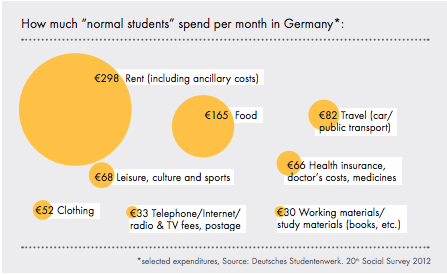
\includegraphics[width=\textwidth,height=150pt]{img/cost.png}
		\begin{center}
			How much “normal students” spend per month in Germany.
		\end{center}
	\end{frame}
	\begin{frame} 
		\frametitle{Funding Models}
	\begin{quotation}
		In 2012, DAAD supported over 4,700 international doctoral students in Germany with scholarships.
	\end{quotation}
		\begin{enumerate}
			\setcounter{enumi}{0}
			\item \textbf{SCHOLARSHIPS}
			\item \textbf{RESEARCH ASSOCIATE JOBS}
			\begin{itemize}
				\item As a rule, doctoral candidates work at the chair of their supervising professor as research associates with temporary part-time contracts.
			\end{itemize}
			\item  \textbf{SIDE JOBS OUTSIDE RESEARCH}
		\end{enumerate} 
	\end{frame}
	\begin{frame} 
		\frametitle{Funding Databases}
		\begin{enumerate}
			\setcounter{enumi}{0}
			\item \textbf{DAAD Scholarship Database}
			\begin{itemize}
				\item German Academic Exchange Service (DAAD) is the largest awarder of scholarships. 
			\end{itemize}
			\item \textbf{EURAXESS Funding Database}
			\begin{itemize}
				\item  Comprises more than 100 programs offered by funding organizations in Germany.
			\end{itemize}
			\item  \textbf{Stipendienlotse}
			\begin{itemize}
				\item Is the database of the Federal Ministry of Education and Research (BMBF) 
			\end{itemize}
		\end{enumerate} 
	\end{frame}
	\section{Conclusion}
	\begin{frame} 
		\frametitle{Conclusion}
		\begin{itemize}
			\item Research in Germany is characterised by an excellent infrastructure, a wide variety of disciplines, well-equipped research facilities and competent staff.\\
			\item Germany offers various forms of research locations: universities, non-university institutes, companies and institutions run by federal or state (“Länder”) authorities.\\
			\item There are more than 800 publicly funded research institutions in Germany, plus research and development (R\&D) centres run by companies.
		\end{itemize}
	\end{frame}
\end{document}